\chapter{Theoretical background}
\label{sec:theory}

The search presented in this thesis is for a simplified model of a supersymmetric theory. The amount of theoretical background required to fully understand this theory can fill many books, and therefore, this document does not attempt to give an exhaustive description of it. Instead, I attempt to give a brief tour of topics that contribute to the understanding of the subject, which are also of personal interest. In addition, I explore the theoretical motivation for supersymmetry, alongside part of the philosophical discussion that normally accompanies such arguments. Whenever possible, I pick a description of a concept that I find intriguing and inspiring in a way that reminds me of my initial spark and inspiration for pursuing a PhD in physics. Good sources for these topics are~\cite{Peskin2019-bt,Srednicki2007-mn}.

\section{Principle of Least Action}
\label{sec:least-action}
The earliest formulation of classical mechanics is normally attributed to the works of Sir Isaac Newton from the 17th century, which is also referred to as Newtonian mechanics. It is based on the then-newly developed mathematics of calculus. A central theorem in calculus is Fermat's theorem, which states that if a function has a local extremum at some point and is differentiable there, then the function's derivative at that point must be zero. The equation of motion is given by Newton's second law, which is an ordinary differential equation given by:
\begin{equation}
\vb{F}=\dv{\vb{p}}{t}=\dv{(m\vb{v})}{t}.
\label{eq:newton-second-law}
\end{equation}
When the mass $m$ is constant, this is equivalent to the famous formula $\vb{F}=m\vb{a}$. In modern physics, a more generalized approach is used based on an \emph{action}. It has been developed in the 18th century, and is able to reproduce Newtonian mechanics, but also to generalize to handle Quantum Mechanics (QM), Relativistic Quantum Field Theory (RQFT) and even General Relativity (GR). The development of that principle was carried out by different people at different times, and can be formulated in equivalent manners. In RQFT, it is useful to use a \emph{Lagrangian}; therefore, it will be shown here rather than the \emph{Hamiltonian} formulation. The two formulations are equivalent, however. Given $N$ generalized coordinates $\vb{q}=\qty(q_1,q_2,\ldots,q_N)$, a \emph{Lagrangian} of the system is written $L\qty( \vb{q}\qty(t), \dot{\vb{q}}\qty(t), t )$, where the dot denotes the time derivative, and $t$ is time. In non-relativistic mechanics for a system of particles in the absence of a magnetic field  $L=T-V$ where $T$ is the total kinetic energy of the system and $V$ is the potential energy of the system. For other systems, writing a Lagrangian is not straightforward, and we assume for now that it is given. The \emph{action} of the system is a functional of the $N$ generalized coordinates, denoted $\mathcal{S}$, given by:
\begin{equation}
\mathcal{S}\qty[ \vb{q}, t_1, t_2 ] = \int^{t_2}_{t_1} L\qty( \vb{q}\qty(t), \dot{\vb{q}}\qty(t), t ) \dd t.
\end{equation}
The principle of least action is then:
\begin{quote}
The path taken by the system between times $t_1$ and $t_2$ and configurations $q_1$ and $q_2$ is the one for which the action is stationary (no change) to first order.
\end{quote}
Mathematically, that is equivalent to requiring $\delta \mathcal{S}=0$ or:
\begin{equation}
\delta \int^{t_2}_{t_1} L\qty( \vb{q}\qty(t), \dot{\vb{q}}\qty(t), t ) \dd t = 0.
\label{eq:principle-of-least-action}
\end{equation}

The principle of least action has been preceded by earlier ideas in optics, such as that for the path of light reflecting from a mirror, the angle of incidence equals the angle of reflection. The principle of least action is the variational equivalent in the calculus of variations of Fermat's theorem in calculus. It is used in order to find a path that extremizes the Lagrangian. Interestingly enough, Fermat also formulated Fermat's principle, which states that "light travels between two given points along the path of shortest time", which is an earlier example of the principle of least action. Using this principle, one can derive the equations of motion of the system. For a classical system, those would be equivalent to  Newton's laws of motion Eq.~\ref{eq:newton-second-law}. Solving Eq.~\ref{eq:principle-of-least-action}, one arrives at Euler–Lagrange equations:
\begin{equation}
\pdv{L}{\vb{q}}-\dv{t}\pdv{L}{\vb{\dot{q}}}=0.
\end{equation}
Solving Euler–Lagrange equations gives the equations of motion of the system. In field theory, an analogous equation is used to calculate the dynamics of a field.

\section{The Quantum}
\label{sec:quantum}

The main object that is the subject of research in particle physics is, of course, a particle. More precisely, an elementary particle or fundamental particle is a subatomic particle that is not composed of other particles. The electron is an example of such a fundamental particle, which was also the first to be discovered by Thomson in 1897. The descriptions and properties of the particles have radically evolved over time, and so did the mathematical language that is used to describe them. In classical electromagnetism, for example, one can use abstractions such as a point charge, point mass, or the concept of an electron as a point using a Dirac delta function $\delta$ in the charge and mass distributions. In quantum mechanics, a wave function $\Psi(\vb{x},t)$ is used, which assigns a complex number to each point $\vb{x}$ at each time $t$. The wave function is governed by the Schrödinger equation~\cite{Liboff2002-vc,Cohen-Tannoudji1977-ms,Cohen-Tannoudji1977-rq}. The time-dependent Schrödinger equation is:
\begin{equation}
i\hbar\pdv{t}\ket{\Psi(t)}=\hat{H}\ket{\Psi(t)}.
\label{eq:schrodinger-eq}
\end{equation}
For a single nonrelativistic particle in one dimension that becomes:
\begin{equation}
i\hbar\pdv{t}\Psi(x,t)=\qty[-\frac{\hbar^2}{2m}\pdv[2]{x}+V(x,t)] \Psi(x,t).
\label{eq:schrodinger-single-eq}
\end{equation}
The parameter $m$ is the mass of the particle, and $V(x,t)$ is the potential that represents the environment in which the particle exists. This can be easily generalized to include more than one particle. However, nonrelativistic quantum mechanics has a shortcoming, in that the Schrödinger equation for massive particles has a fixed number of particles governing the state of the system. It is not surprising given the fact that in classical mechanics, and therefore nonrelativistic quantum mechanics by extension, mass is never created nor destroyed. In order to accommodate the observation that particles are being created and destroyed, a relativistic treatment is needed. That is the goal of RQFT.

But the equivalent of particles does actually arise in nonrelativistic quantum mechanics: when they are massless. In fact, the formalism for creating and destroying massless particles, known as quanta, is generalized from quantum mechanics to RQFT. The quantum arises in the quantum mechanical harmonic oscillator. Classically, a harmonic oscillator is a system that, when displaced from its equilibrium position, experiences a restoring force $F$ proportional to the displacement $x$:
\begin{equation}
\vb{F}=-k\vb{x},
\end{equation}
where $k$ is a positive constant. The potential energy stored in a simple harmonic oscillator at position $x$ is:
\begin{equation}
U=\frac{1}{2}kx^2.
\end{equation}
Writing a Hamiltonian and promoting the observables to operators we get:
\begin{equation}
\hat{H} = \frac{\hat{p}^2}{2m} + \frac{1}{2}k\hat{x}^2 = \frac{\hat{p}^2}{2m} + \frac{1}{2}m\omega^2 \hat{x}^2,
\end{equation}
where $m$ is the particle's mass, $k$ is the force constant, $\omega = \sqrt{k/m}$ is the angular frequency of the oscillator, $\hat{x}$ is the position operator, and $\hat{p}$ is the momentum operator. Solving the time-independent Schr{\"o}dinger equation gives the energy levels
\begin{equation}
E_n=\hbar\omega\qty(n+\frac{1}{2})=\qty(2n+1)\frac{\hbar}{2}\omega.
\end{equation}
It is interesting to note that the energies are quantized and equally spaced with discrete energy values of integer-plus-half multiples of $\hbar\omega$.

\subsection{Annihilation and Creation Operators}
\label{sec:ladder-operators}
We define ladder operators
\begin{equation}
\begin{split}
\hat{a} &\equiv \sqrt{\frac{m\omega}{2\hbar}} \left(  \hat{x} + \frac{i\hat{p}}{m\omega_0}  \right) \\
\hat{a}^\dagger &\equiv \sqrt{\frac{m\omega}{2\hbar}}\left(  \hat{x} - \frac{i\hat{p}}{m\omega_0}  \right).
\end{split}\label{ac}
\end{equation}
As can be seen, $\hat{a}$ is not Hermitian. 
Using $\left[ \hat{x}, \hat{p}  \right] = i\hbar$ it is easy to show that
\begin{equation}\label{acom}
\begin{split}
&\left[ \hat{a}, \hat{a}^\dagger  \right] = 1\\
&\hat{a} \hat{a}^\dagger = 1 + \hat{a}^\dagger  \hat{a}.
\end{split}
\end{equation}
By reversing \ref{ac} we get
\begin{equation}\label{xho}
\hat{x} = \sqrt{\frac{\hbar}{2m\omega}}\qty(\hat{a} + \hat{a}^\dagger)\, ,\qquad
\hat{p} = i\sqrt{\frac{\hbar m \omega}{2}} \qty(\hat{a} - \hat{a}^\dagger)
\end{equation}
and the Hemiltonian becomes
\begin{equation}
\hat{H} = \hbar\omega_0\left(  \hat{a}^\dagger  \hat{a}+ \frac{1}{2} \right) \equiv \hbar\omega_0\left( \hat{N} + \frac{1}{2} \right).
\end{equation}
Finding eigenvalues for $\hat{H}$ becomes finding eigenvalues of the \emph{number operator} $\hat{N} \equiv  \hat{a}^\dagger  \hat{a}$, which are
\begin{equation}
N\ket{n}=n\ket{n}.
\end{equation}
Operating with the ladder operators on the energy eigenstates gives
\begin{equation}
\begin{split}
\hat{a}^\dagger \ket{n} &= \sqrt{n+1}\ket{n+1}\\
\hat{a}\ket{n} &= \sqrt{n}\ket{n-1}.
\end{split}
\end{equation}
It is seen that $\hat{a}^\dagger$, in essence, appends a single quantum of energy to the oscillator, while $\hat{a}$ removes a quantum. Furthermore, acting with the number operator $\hat{N}$ yields
\begin{equation}
\begin{split}
N\hat{a}^\dagger \ket{n} &= (n+1)\hat{a}^\dagger\ket{n} \\
N\hat{a}\ket{n} &= (n-1)\hat{a}\ket{n}.
\end{split}
\end{equation}
Due to this, $\hat{a}$ is called annihilation operator ("lowering operator"), and $\hat{a}^\dagger$ creation operator ("raising operator"). The two operators together are called ladder operators. In quantum field theory, these operators destroy and create particles, which correspond here to a quanta of energy of $\hbar\omega$.

\section{Relativistic Quantum Field Theory}
\label{sec:rqft}

In the first quarter of the twentieth century, two of the most successful theories in modern physics were developed: special relativity and quantum mechanics. Special relativity was necessary to solve the incompatibility between Maxwell's equations of electromagnetism and Newtonian mechanics. In addition, experimentally, the null result of the Michelson–Morley experiment demonstrated that the historically hypothesized aether did not exist. Special relativity diverges from classical mechanics at high-velocities. Quantum mechanics, on the other hand, arose gradually from theories that aimed to explain observations that could not be reconciled with classical physics, such as Max Planck's solution to the black-body radiation problem and the correspondence between energy and frequency in Albert Einstein's photoelectric effect. Quantum mechanics differs from classical physics in several aspects: energy, angular momentum, and other quantities of a bound system are restricted to discrete values; objects have characteristics of both particles and waves; and there are limits to how accurately the value of a physical quantity can be predicted prior to its measurement, given a complete set of initial conditions (the uncertainty principle).

Since classical mechanics diverged into two different directions, namely, quantum mechanics and special relativity (which later on developed further into general relativity, but that's beyond the concern here), it was clear that a theory that incorporates both developments is needed. The first effort came from an attempt in creating a quantum mechanical theory of the electromagnetic field. It was also crucial to develop a theory, in which the number of particles changes, in order describe processes such as a $\beta$-decay or the emission of a photon by an electron dropping into a quantum state of lower energy in an atom.

Quantum field theory successfully combines classical field theory, special relativity, and quantum mechanics. QFT treats particles as excited states (also called quanta) of their underlying quantum fields, which are more fundamental than the particles. The equation of motion of the particle is determined by minimization of the Lagrangian, a functional of fields associated with the particle. Interactions between particles are described by interaction terms in the Lagrangian involving their corresponding quantum fields. Each interaction can be visually represented by Feynman diagrams according to perturbation theory in quantum mechanics.

\subsection{Attempts at Relativistic Quantum Mechanics}
\label{sec:attempts-rqt}

At first glance, fields are not the only way to try and reconcile quantum mechanics and relativity. A naive attempt~\cite{Srednicki2007-mn} could be to take the Schrödinger equation~\ref{eq:schrodinger-eq} and write a Hamiltonian in a relativistic notion $H=\sqrt{\hat{\vb{p}}^2+m^2}$ (taking as usual $\hbar=c=1$). Plugging it as is into the Schrödinger equation will result in the time derivative outside the square root, while the space derivatives under it, which is not in the spirits of relativity. Squaring the differential operators before applying them to the wave function and collecting terms results in the \emph{Klein-Gordon equation}:
\begin{equation}
\qty(\pdv[2]{t}-\nabla^2+m^2)\Psi\qty(\vb{x},t)=0.
\label{eq:kg-wf}
\end{equation}
It is second-order in both space and time derivatives, and they appear in a symmetric fashion. The $\Psi$ in the equation is the usual quantum mechanical wave function. There are two problems with sticking to the wave function. The first is that the norm of a state $\braket{\Psi,t}$ is not in general time independent. Thus probability is not conserved. The Klein-Gordon equation obeys relativity, but not quantum mechanics. This specific problem is solved (for spin-one-half particles) by the \emph{Dirac equation}. In its original form written by Dirac~\cite{Dirac1981-rt}:
\begin{equation}
\qty(\beta m c^2 + c\sum^3_{n=1}\alpha_n p_n)\Psi\qty(\vb{x},t)=i\hbar\pdv{\Psi\qty(\vb{x},t)}{t}
\label{eq:dirac-wf}
\end{equation}
where $\Psi\qty(\vb{x},t)$ again is to be interpreted as an ordinary quantum mechanical wave function for the electron of rest mass $m$ with spacetime coordinates $x, t$. The $p_1,p_2,p_3$ are the components of the momentum, understood to be the momentum operator in the Schrödinger equation. The new elements in this equation are the four $4\times 4$ matrices $\alpha_1,\alpha_2\alpha_3$ and $\beta$, and the four-component wave function $\Psi$. There are four components in $\Psi$ because the evaluation of it at any given point in configuration space is a bispinor. It is interpreted as a superposition of a spin-up electron, a spin-down electron, a spin-up positron, and a spin-down positron. The $4\times 4$ matrices $\alpha_k$ and $\beta$ are all Hermitian and satisfy:
\begin{equation}
\alpha_i^2=\beta^2=I_4,
\end{equation}
and they all mutually anticommute:
\begin{equation}
\begin{split}
&\alpha_i \alpha_j + \alpha_j \alpha_i = 0 \:(i\neq j) \\
&\alpha_i \beta + \beta \alpha_i = 0.
\end{split}
\end{equation}
It turns out that the Dirac equation is fully consistent with relativity. However, there are some problems. The minimum size of the matrices of $4\times 4$ implies two additional "spin" states. They also imply negative eigenvalues for the Hamiltonian, which indicates that there is no ground state. Dirac postulated his famous \emph{Dirac sea} of electrons to suggest that the negative energy states are all occupied. An electron in the sea could then be excited to a positive energy state, leaving behind a \emph{hole} in the Dirac sea. This hole would appear to have positive charge, and positive energy. Dirac therefore predicted (in 1927) the existence of the positron, a particle with the same mass as the electron, but opposite charge. The positron was found experimentally five years later.

The problem with this solution though, is that we've started by trying to describe a theory of a single half-spin particle, and ended up describing a theory with infinite amount of particles. Even if this is taken to be satisfactory, this theory still cannot describe particles that do not obey Pauli exclusion, such as photons or pions. The problem lies in the difference between the way that nonrelativistic quantum mechanics and special relativity treats space and time. In special relativity, space and time are treated on equal footing. In nonrelativistic quantum mechanics, however, space is an operator, while time isn't. It turns out that turning time into an operator is a very difficult problem. The approach that proved to be fruitful is to make space a \emph{label}, just as time is, by turning the wave function $\Psi$ into a \emph{field}. Space and time are now labels in a \emph{quantum field} $\varphi(\vb{x},t)$ of operators. Each point in space and time now point to an operator. This allows one to really treat space and time on an equal footing.

\subsection{Classical Field Theory}
\label{sec:classical-field}

After the naive attempts at a relativistic quantum mechanics introduced in Section~\ref{sec:attempts-rqt}, two successful and widely used methods of constructing quantum field theories are described in Section~\ref{sec:quantization}. The first is the canonical quantization in Section~\ref{sec:canonical}, and the second is the path integrals formalism in Section~\ref{sec:path-integrals}. They involve starting from a classical field theory and quantizing it. In a classical field theory, the equation of motion can be derived from variation of an action $\mathcal{S}=\int \dd{t}L$, where $L$ is the Lagrangian, which is the spatial integral of a Lagrangian density $\mathcal{L}$, so that $L=\int \dd[3]x\mathcal{L}$. The Lagrangian density is a function of one or more fields $\phi(x)$, and their derivatives $\partial_{\mu}\phi$, so that
\begin{equation}
\mathcal{S}=\int \dd{t}L=\int \mathcal{L}\qty(\phi,\partial_{\mu}\phi)\dd[4]x.
\end{equation}
Following the principle of least action described in Section~\ref{sec:least-action}, we  take the action $\mathcal{S}$ to an extremum and write
\begin{equation}
\begin{split}
0 & =  \delta \mathcal{S} \\
& = \int \mathrm{d}^4 x \left\lbrace \frac{\partial\mathcal{L}}{\partial\phi}\delta\phi + \frac{\partial\mathcal{L}}{\partial\left(\partial_\mu\phi\right)}\delta\left(\partial_\mu\phi\right) \right\rbrace \\
& = \int \mathrm{d}^4 x \left\lbrace \frac{\partial\mathcal{L}}{\partial\phi}\delta\phi - \partial_\mu \left(   \frac{\partial\mathcal{L}}{\partial\left(\partial_\mu\phi\right)} \right) \delta\phi   +   \partial_\mu \left(   \frac{\partial\mathcal{L}}{\partial\left(\partial_\mu\phi\right)}  \delta\phi \right) \right\rbrace .
\end{split}
\end{equation}
The last term can be turned into a surface integral over the boundary of the region of integration. Since $\delta\phi$ vanish on the spatial boundary, the surface term is zero. After rearrangement, we arrive at the Euler-Lagrange equation of motion for a field,  
\begin{equation}
\partial_\mu \left(   \frac{\partial\mathcal{L}}{\partial\left(\partial_\mu\phi\right)} \right) - \frac{\partial\mathcal{L}}{\partial\phi} = 0 .
\end{equation}
If the Lagrangian contains more than one field, there is one such equation for each. The Hamiltonian of a discrete system can be written as
\begin{equation}
H \equiv \sum p\dot{q} - L,
\end{equation}
where $q$ is a dynamical variable, and $p\equiv \pdv*{L}{\dot{q}}$ is the conjugate momentum. To generalize to continuous system we define the \emph{momentum density} conjugate to $\phi\qty(\vb{x})$ as
\begin{equation}
\pi\qty(\vb{x})\equiv\pdv{\mathcal{L}}{\dot{\phi}\qty(\vb{x})},
\end{equation}
and the Hamiltonian can be expressed, using the Hamiltonian desnsity $\mathcal{H}$ as:
\begin{equation}
H = \int \mathrm{d}^3x [\pi(\mathbf{x})\dot{\phi}(\mathbf{x}) - \mathcal{L}] \equiv \int \mathrm{d}^3x \mathcal{H} .
\end{equation}
As an example, consider the theory of a single real scalar field $\phi\qty(x)$ with the Lagrangian
\begin{equation}
\mathcal{L} = \frac{1}{2}\left( \partial_\mu \phi \right)^2-\frac{1}{2}m^2\phi^2.
\label{eq:kg-lagrangian}
\end{equation}
Following the usual procedure and applying the Euler-Lagrange equation gives the equation of motion
\begin{equation}
\left(\partial^\mu\partial_\mu + m^2\right)\phi=0,
\end{equation}
which is the well-known Klein-Gordon equation. Here, $\phi$ is a classical field, and not a wave function, nor a quantum field. The Hamiltonian that results from the procedure described above is
\begin{equation}
H = \int \mathrm{d}^3x\left[ \frac{1}{2}\pi^2 + \frac{1}{2}\left( \nabla\phi \right)^2 + \frac{1}{2}m^2\phi^2  \right].
\end{equation}

\subsection{Quantization}
\label{sec:quantization}

As described in Section~\ref{sec:classical-field}, two methods of constructing quantum field theories are widely used. The first is the canonical quantization in Section~\ref{sec:canonical}, and the second is the path integrals formalism in Section~\ref{sec:path-integrals}. The path integrals formalism has an advantage in that it uses the Lagrangian formalism rather than the Hamiltonian. The Lagrangian formalism is explicitly Lorentz invariant, and in general, it is in practice easier to guess the correct form of the Lagrangian of a theory, which naturally enters the path integrals than the Hamiltonian. The advantage of the canonical quantization is that unitarity of the S-matrix is more explicit than in the path integral approach. The methods are described here in a very qualitatively manner. For an explicit mathematical formulation, Ref.~\cite{Peskin2019-bt,Srednicki2007-mn} are great sources for that.

\subsubsection{Canonical Quantization}
\label{sec:canonical}

Canonical quantization starts with a classical field theory, and \emph{quantized} by promoting the dynamical variables to operators that obey canonical commutation relations. It can be demonstrated with the example of the Klein-Gordon case, which has the classical Lagrangian~\ref{eq:kg-lagrangian}. Promoting the field and momentum density to operators, the commutation relations generalize to:
\begin{equation}
\begin{split}
\comm{\phi\qty(\vb{x})}{\pi\qty(\vb{y})}&=i\delta^{(3)}\qty(\vb{x}-\vb{y});\\
\comm{\phi\qty(\vb{x})}{\phi\qty(\vb{y})}&=\comm{\pi\qty(\vb{x})}{\pi\qty(\vb{y})}=0.
\end{split}
\end{equation}
Writing the Klein-Gordon equation in Fourier space, one gets:
\begin{equation}
\qty[\pdv[2]{t} + \qty(\abs{\vb{p}}^2+m^2)]\phi(\vb{p},t)=0.
\end{equation}
This is the same as the equation of motion for a simple harmonic oscillator with the frequency $\omega_{\vb{p}}=\sqrt{\abs{\vb{p}^2+m^2}}$. Therefore a similar treatment as in  Section~\ref{sec:quantum} can be done here. Ladder operators are introduced, only that now each Fourier mode of the field is treated as an independent oscillator with it own $a$ and $a^\dagger$. The spectrum of the Klein-Gordon Hamiltonian can then be found in the same manner, and can be written as:
\begin{equation}
H=\int \frac{\dd^2 p}{(2\pi)^3} \omega_{\vb{p}}\qty(a^\dagger_{\vb{p}}a_{\vb{p}}+\frac{1}{2}\comm{a_{\vb{p}}}{a^\dagger_{\vb{p}}}).
\end{equation}
The operator $a^\dagger_{\vb{p}}$ created a particle with momentum $\vb{p}$ and energy $\omega_{\vb{p}}=\sqrt{\abs{\vb{p}^2+m^2}}$. The particles follow the proper relativistic energy-momentum relation, and have strictly positive energy. Since $a^\dagger_{\vb{p}}$ and $a^\dagger_{\vb{q}}$ commute, two particles are interchangeable. Moreover, since arbitrarily many particles can be produced for a single mode $\vb{p}$, the particles obey \emph{Bose-Einstein statistics}. In a theory of half-integer spin particles, anticommutators are to be used. The next steps in this formalism is to compute correlation functions, and eventually write down the full Feynman rules for the theory, in order to compute cross sections and decay rates.

\subsubsection{Path Integrals}
\label{sec:path-integrals}

The path integral formalism is an alternative construction to quantum mechanics developed by Richard Feynman, and is proven to be equivalent to the wave equation of Schrödinger, and the matrix algebra of Heisenberg, Born and Jordan. It is also used as an alternative way to construct quantum field theories, as an alternative to the canonical quantization. Using this formalism, it is easier to compute propagators and derive Feynman rules. It also generalizes better to non-Abelian gauge theories. Moreover, since it uses the Lagrangian, rather than the Hamiltonian, as its fundamental quantity, it explicitly preserves all symmetries of a theory. Using path integrals allows the direct computation of the scattering amplitude of a certain interaction process, rather than the establishment of operators and state spaces. 

Suppose we are interested to compute the amplitude for a particle to travel from one point $x_a$ to another $x_b$ in a given time $T$. The amplitude $U\qty(x_a,x_b,T)$ in the canonical Hamiltonian formalism, using the time evolution operator, is given by
\begin{equation}
U\qty(x_a,x_b,T)=\mel{x_b}{e^{-iHT/\hbar}}{x_a}.
\end{equation}
In the path integral approach, the total time T is divided into N small intervals, and the overall amplitude is the product of the amplitude of evolution within each interval, integrated over all intermediate states. The propagation amplitude becomes:
\begin{equation}
\mel{x_b}{e^{-iHT/\hbar}}{x_a}=U\qty(x_a,x_b,T)=\int \mathcal{D}x(t)e^{iS\qty[x(t)]/\hbar},
\end{equation}
where $S\qty[x(t)]$ is the classical action, and $\int \mathcal{D}x(t)$ is another way of writing "sum over all paths". This functional formula then allows for the calculation of correlation functions and eventually writing down the full Feynman rules for the theory.

\subsection{Interactions}

The goal of every scientific theory is to make predictions about measurements. In the context of QFT, it is normally one of two generic cases: one incoming particle, for which a decay rate is computed, or two incoming particles, for which a cross section is computed. For this, a recipe for computing a scattering amplitude and converting it into a measurable quantity is needed.

\subsubsection{The Cross Section and Decay Rate}
\label{sec:cross-section}

The \emph{cross section} is the likelihood of any particular final state from the collusion of two beams of particles with well-defined momenta. The \emph{cross section}, which has the units of area and is denoted by $\sigma$, is proportional to the total number of events (of whatever desired type):
\begin{equation}
\sigma \equiv \frac{\text{Number of scattering events}}{\rho_\mathcal{A}\,l_\mathcal{A}\,\rho_\mathcal{B}\,l_\mathcal{B}\,A}
\end{equation}
where $\mathcal{A}$ are particles at rest with density $\rho_\mathcal{A}$, aimed by particles of type $\mathcal{B}$ with density $\rho_\mathcal{B}$ with velocity $v$, and $l_\mathcal{A}$ and $l_\mathcal{B}$ are the lengths of the bunches of particles. $A$ is the cross-sectional area common to the two bunches. We get
\begin{equation}
\text{Number of events} = \sigma\,l_\mathcal{A}\,l_\mathcal{B}\int d^2 x\,\, \rho_\mathcal{A}(x)\,\rho_\mathcal{B}(x)
\end{equation}
The \emph{differential cross section} is $d\sigma/(d^3 p_1\ldots d^3p_n)$ which when integrated over any small $d^3 p_1\ldots d^3p_n$ gives the cross section for scattering into that region of final-state momentum space. Cross sections are computed for a production of a specific process. The \emph{decay rate} $\Gamma$ of an unstable particle $\mathcal{A}$ assumed to be at rest into a specified final state is defined as
\begin{equation}
\Gamma \equiv \frac{\text{Number of decays per unit time}}{\text{Number of $\mathcal{A}$ particles present}}.
\end{equation}

\subsubsection{Interacting Fields}

The example that was used in previous sections, the Klein-Gordon field, was a free field theory. No interactions and no scattering were involved. In reality, particles do interact and scatter of each other. In order to obtain such interactions, nonlinear terms must added to the Lagrangian. One example of such an interacting Lagrangian is the "phi-fourth" theory,
\begin{equation}
\mathcal{L} = \frac{1}{2}(\partial_\mu\phi)^2-\frac{1}{2}m^2\phi^2 -\frac{\lambda}{4!}\phi^4
\end{equation}
where $\lambda$ is a dimensionless \emph{coupling constant}. The goal is to be able to compute scattering amplitudes for an interacting theory, in order to convert them into cross sections. This is generally impossible to solve exactly. Instead it is computed in the framework of \emph{perturbation theory}. It turns out that the perturbation series is quite simple in structure, and can be visualized with the use of \emph{Feynman diagrams}.

\subsection{Feynman Diagrams}

In order to compute cross sections and decay rates, one must compute matrix elements of the S-matrix. The S-matrix gives the probability amplitude for a scattering event between \emph{in} and \emph{out} states. The probability amplitude for producing the final state is simply related to the cross section. Computing the S-matrix elements, or scattering amplitudes, is done differently depending on the quantization scheme, canonical or path integrals. As previously mentioned, the computation is done in a perturbation series. A Feynman diagram is a graphical representation of a perturbative contribution to the transition amplitude or correlation function. In the canonical quantization, a Feynman diagram represents a term in the Wick expansion of the perturbative S-matrix. 

The quantization scheme also provides \emph{Feynman rules} in order to compute the value of each Feynman diagram. It involves providing a mathematical expression for a \emph{propagator} for each internal line, or virtual particle. Each diagram then has an amplitude, which is a term in the perturbative expansion. In Figure~\ref{fig:e-to-mu-feynman}, an example of a tree-level diagram representing a process of $e^+ e^- \rightarrow \mu^+ \mu^-$ through a photon $\gamma$ is shown.

\begin{figure}[!htb]
\centering
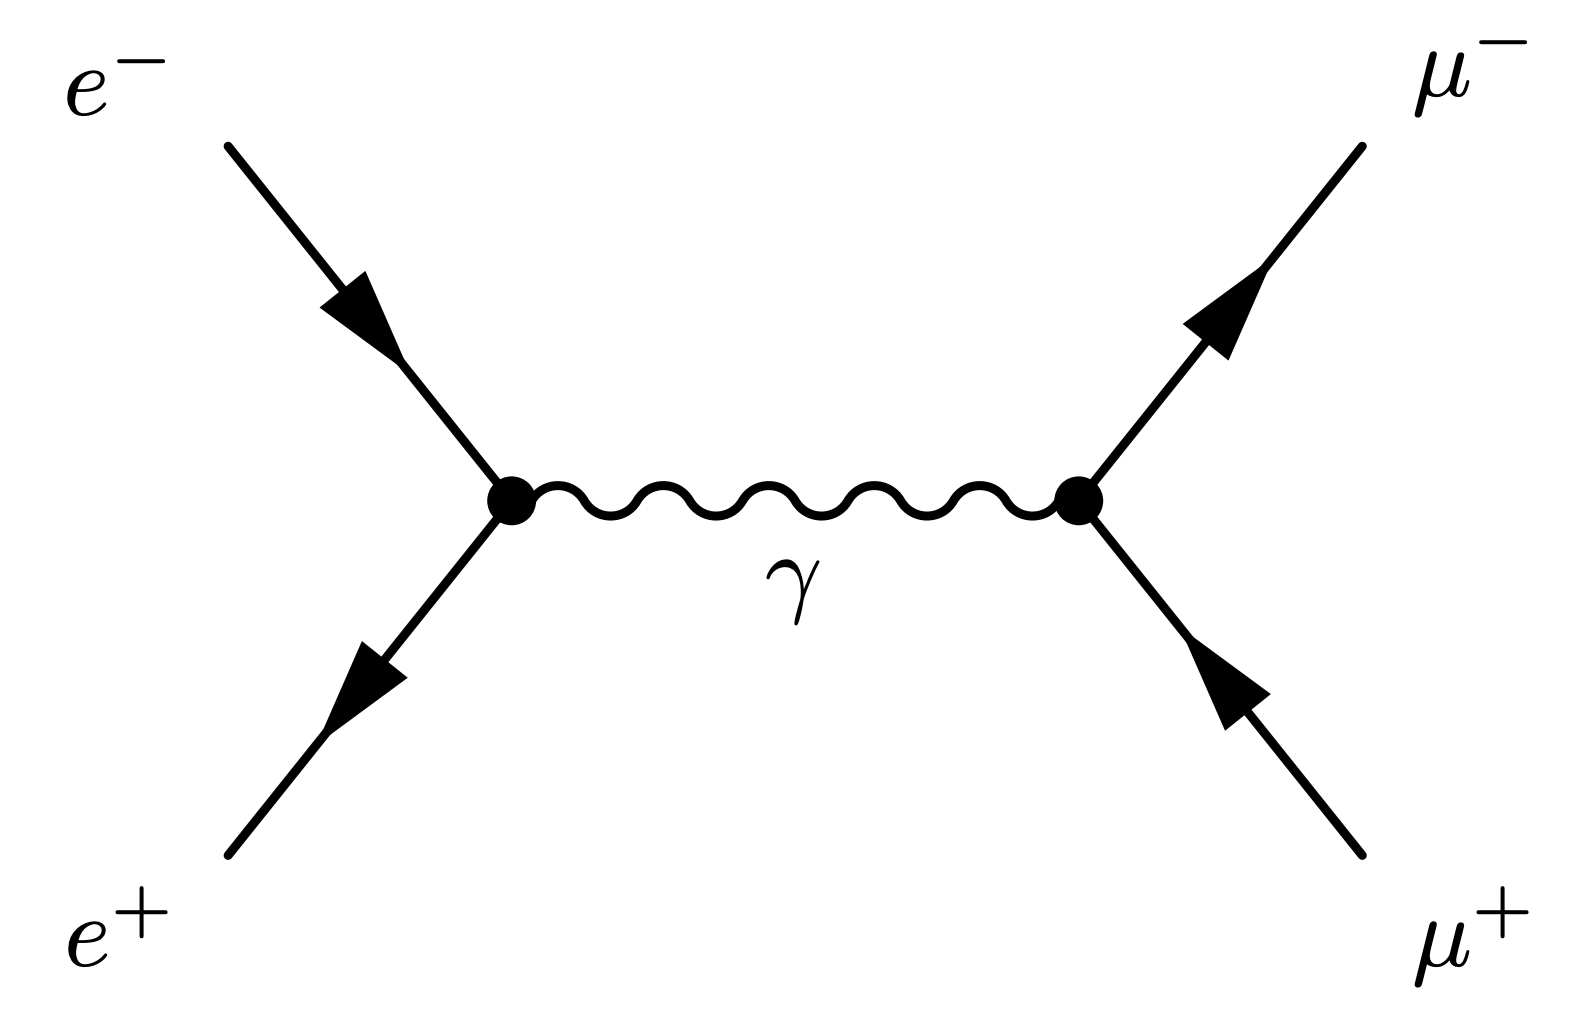
\includegraphics[width=0.5\linewidth]{plots/feynman_diagrams/feynman_e_to_mu.png}  \\
\caption[Electrons to Muons Feynman diagram]{Feynman diagram representing the tree-level process of $e^+ e^- \rightarrow \mu^+ \mu^-$. Electron and positron annihilate each other and produce muon-antimuon pair through a virtual photon.}
\label{fig:e-to-mu-feynman}
\end{figure}

\clearpage
\section{Symmetries}

In 1964, Richard Feynman gave a series of seven lectures called \emph{The Character of Physical Laws} at Cornell University, as part of the Messenger Lectures series. The lectures were videotaped by the BBC, and are available online alongside their transcripts~\cite{Feynman1997-vo}. It is such a precious piece of history, and I would recommend everyone to watch it, as it is meant for the public audience. It showcases not only Feynman's ability to explain complex ideas and theories, but also his funny and enchanting personality. The fourth lecture in that series is called \emph{Symmetry in Physical Laws}, in which he starts by describing how Weyl defines a symmetry:

\begin{quote}
So, Weyl said, a thing is symmetrical if there’s something that you can do to it, so that after you’re finished doing it, it looks the same as it did before. That is the sense in which we say that the laws of physics are symmetrical: that there are things that we can do to the physical laws, or to our way of representing the physical laws, which make no difference and leave everything unchanged in its effects.
\end{quote}

Most physicists will probably agree that's what they mean when they say that a physical law is symmetrical. In this chapter, we are concerned with symmetries of laws, rather than symmetries of objects, such as a human face, for example. In modern physics, largely thanks to Noether's theorem, symmetries became fundamental, and they set the foundations of the Standard Model of particle physics. In this chapter, I summarize the reasons why symmetries are so important and what roles they play in the Standard Model. But first, I would like to introduce my favorite physics riddle, which Feynman described, starting at minute 40:04 in the same lecture:

\begin{quote}
Suppose that we were in telephone conversation with a Martian or an Arcturian, or something. We don’t know where he is and we would like to describe things to him. We want to tell him about things. You say, so how’s he going to understand the words, well, that’s been studied very much by Professor Morrison here. He has pointed out that one way would be to start out and say tick tick two, tick tick tick three, and so on, and pretty soon the guy’d catch onto the numbers. Then—as he understands your number system, then—you can write lots of numbers and you could, for example, write a whole sequence of numbers that represents the weights, the proportional weights, of the different atoms, in succession.

Then say, hydrogen: 1.008, deuterium, and so on and so on. And he would-after he sat down with all those numbers and piddled around a while, would-discover that the mathematical ratios were the same as the ratios of the weights of the elements and, therefore, those names must be for the elements—and so gradually, you could, in talking to him, have a common language, in many ways, common. There are many-now comes the problem.

Suppose that he says, you fellas—after we get familiar with him, he says, "You’re very nice; now I’d like to know what you look like." And you start out, "Well, we’re about six feet tall." He says, "Six feet, how big is a foot?" "It’s very easy," you say; "six feet tall is 170 thousand million hydrogen atoms high." Well, it’s not a joke; it’s a possible way of describing six feet to someone that has no measure, assuming that we cannot send him any samples, nor can we both look at the same object.

If we have to tell him how big we are; we can do it. That’s because the laws of physics are not unchanged under a scale change. We can use that factor, use the properties of the scale to determine—I mean, you can use that fact to determine the scale.

Well, here we’ve described ourselves after telling six feet tall, and we’re so-and-so bilateral on the outside, and we look like this, and there are these prongs sticking out, and all this. And he says, "That’s very interesting; what do you look like on the inside?" So we describe the heart and so on, and we say, "Now, put the heart in on the left side."

Now the question is, how can we tell him which side is the left side?
\end{quote}

To put it shortly, the riddle is how to communicate the concept of left and right via radio signals to an alien civilization without reference to common sightings. Most physicists attempt to solve this problem by thinking of the right-hand rule in electromagnetism. Unfortunately, that would not work. The correct solution is very unexpected and one of the most surprising results of modern physics. The solution is explained in the section about discrete symmetries~\ref{sec:discrete-symmetries}.

\subsection{Conservation Laws}

A conservation law states that a particular measurable property of an isolated physical system does not change as the system evolves over time. Conservation laws are useful because they describe which processes can or cannot occur in nature. They also allow properties of the motion to be derived without solving the equations of motion. Conservation laws have changed throughout history, and some are a part of one theory but not another. Mass, for example, is conserved in classical mechanics, but not in relativity due to the principle of mass–energy equivalence. However, it is a good approximation when the assumptions of classical mechanics hold, such as low velocities and energies, and large enough objects. Most conservation laws are exact, or absolute, in the sense that they apply to all possible processes. Some conservation laws are partial, in that they hold for some processes but not for others.

In continuum mechanics, the most general form of an exact conservation law is given by a continuity equation. For example, conservation of electric charge $q$ is
\begin{equation}
\pdv{\rho}{t}=-\nabla\cdot\vb{j},
\end{equation}
where $\rho$ is the density of $q$ (amount per unit volume), $\vb{j}$ is the flux of $q$ (amount crossing a unit area in unit time), and $t$ is time. There are several methods for identifying conservation laws. It can be hypothesized and proved mathematically. In classical mechanics, Hamilton–Jacobi equations provide a method for identifying constants of motion, and so does Poisson's theorem. In QM, an observable quantity $Q$ will be a constant of motion if it commutes with the Hamiltonian, and it does not itself depend explicitly on time. In the context of particle physics, the most powerful theorem invoked in order to study conservation laws is Noether's theorem~\ref{sec:noethers-theorem}. It is also this theorem that connects conservation laws to symmetries, which is the topic of this section.

Currently, exact conservation laws that have never been proven to be violated include conservation of mass-energy $E$, conservation of linear momentum $\vb{p}$, conservation of angular momentum $\vb{L}$, conservation of electric charge, conservation of weak isospin, conservation of color charge, and conservation of CPT parity. Approximate conservation laws, \ie, conservation laws which are approximately true in particular situations, such as low speeds, short time scales, or certain interactions include conservation of mechanical energy, mass, flavor, strangeness, space-parity, charge-parity, time-parity, and CP parity.

\subsection{Noether's Theorem}
\label{sec:noethers-theorem}

In 1915, German-Jewish female mathematician Amalie Emmy Noether proved one of the most fundamental theorems of 20th-century modern physics. In the spring of that year, she was invited by David Hilbert and Felix Klein to join the Göttingen mathematics department, challenging the views of some of his colleagues that a woman should not be allowed to teach at a university. Soon after arriving at Göttingen, she demonstrated her capabilities by proving the theorem now known as Noether's theorem, which shows that a conservation law is associated with any differentiable symmetry of a physical system~\cite{Lederman2004-fl}. That made modern theoretical physicists much more focused on symmetries.

Informally, Noether's theorem can be stated as:
\begin{quote}
If a system has a continuous symmetry property, then there are corresponding quantities whose values are conserved in time.
\end{quote}
In the context of classical field theory, it can be stated as:
\begin{quote}
To each differentiable symmetry of a local Lagrangian, there corresponds a conserved current.
\end{quote}
Previously, we described a symmetry as something that you can do to a system, so that it looks the same as it did before. More formally in this context, a symmetry is the covariance of the form that a physical law takes, where by covariance, we mean the invariance of the form of physical laws under differentiable transformations. That means continuous transformations that leave the equations of motion invariant. Formally, in the context of classical field theories, the theorem can be stated in the language of fields~\cite{Peskin2019-bt}. Consider a continuous transformations on the fields $\phi$, which in infinitesimal form can be written
\begin{equation}
\phi(x)\rightarrow\phi^\prime(x)=\phi(x)+\alpha\Delta\phi(x),
\label{eq:infi-trans}
\end{equation}  
where $\alpha$ is an infinitesimal parameter and $\Delta\phi(x)$ is some deformation of the field configuration. It is considered a symmetry if it leaves the equations of motion invariant. This is ensured either if the action is invariant under the transformation or if it is changed by a surface term. The Lagrangian, therefore, must be invariant under  the transformation in Equation~\ref{eq:infi-trans} up to a 4-divergence:
\begin{equation}
\mathcal{L}(x)\rightarrow\mathcal{L}(x)+\alpha\partial_{\mu}\mathcal{J}^{\mu}(x),
\end{equation}
for some $\mathcal{J}^{\mu}$. After varying the fields, one finds:
\begin{equation}
\partial_{\mu}j^{\mu}=0,\qquad \textrm{for} \quad j^{\mu}(x)=\pdv{\mathcal{L}}{\qty(\partial_{\mu}\phi)}\Delta\phi-\mathcal{J}^{\mu}.
\end{equation}
This result states that the current $j^{\mu}(x)$ is conserved. This can also be expressed by saying that the charge
\begin{equation}
Q\equiv\int_{\textrm{all space}}j^0\dd[3]{x}
\end{equation}
is a constant in time.

\clearpage
\subsection{Groups}

We have seen that symmetries lead to conservation laws via Noether's theorem. Intuitively, we stated that symmetries are things that don't change while other things do change. The mathematical description of symmetries is Group Theory~\cite{Robinson2011-dv}. Groups are fundamental in particle physics, since they describe the symmetries which the laws of physics seem to obey. The first example encountered in particle physics is Lorentz covariance, or Lorentz symmetry. It is an equivalence of observation or observational symmetry due to special relativity, implying that the laws of physics stay the same for all observers that are moving with respect to one another within an inertial frame. Mathematically speaking, a physical quantity is said to be Lorentz covariant if it transforms under a given representation of the Lorentz group. In particular, a Lorentz covariant scalar (\ie, the space-time interval) remains the same under Lorentz transformations and is said to be a Lorentz invariant. Another important example is gauge theories. A gauge theory is a type of field theory in which the Lagrangian does not change (is invariant) under local transformations according to certain smooth families of operations (Lie groups).

A \emph{Group}, denoted $\qty(G, \star)$, is a set of object, denoted $G$, and some operation on those objects, denoted $\star$, subject to the following:
\begin{enumerate}
\item For any two elements $g_1$ and $g_2$ in $G$, the elemet $g_1\star g_2$ is also in $G$. This property is called \emph{closure}.
\item For any three elements $g_1, g_2$ and $g_3$ in $G$, the relation $\qty(g_1\star g_2)\star g_3=g_1\star\qty(g_2\star g_3)$ must hold. This property is called \emph{associativity}.
\item There exists an element of $G$ which we will denote $e$, that satisfies $e\star g = g\star e = g$ for every element $g$ of $G$. This property is called \emph{identity}.
\item For every element $g$ of $G$, there is another element of $G$ which we will denote $g^{-1}$ that satisfies $g^{-1}\star g = g\star g^{-1}=e$. This property is called \emph{inverse}.
\end{enumerate}
A group in which $g_i\star g_j=g_j\star g_i$ is called \emph{abelian}. Otherwise, it is non-abelian. Groups can be \emph{discrete} or \emph{continuous}. We will mainly concern ourselves with continuous groups. It is easy to see that Lorenz transformations and gauge transformation form continuous groups.

A \emph{representation} of a group $G$ on a vector space $V$ over a field $K$ is a group homomorphism from $G$ to $GL(V)$, the general linear group on $V$. That is, a representation is a map
\begin{equation}
\rho:G\rightarrow GL(V)
\end{equation}
such that
\begin{equation}
\rho\qty(g_1 g_2)=\rho\qty(g_1)\rho\qty(g_2),\qquad \textrm{for all}\,\, g_1,g_2\in G.
\end{equation}
In other words, a representation assigns a matrix to each element of the group, while the operation is represented by regular matrix multiplication and preserves the group multiplication table. A subspace $W$ of $V$ that is invariant under the group action is called a \emph{subrepresentation}. If $V$ has exactly two subrepresentations, namely the zero-dimensional subspace and $V$ itself, then the representation is said to be \emph{irreducible}; if it has a proper subrepresentation of nonzero dimension, the representation is said to be \emph{reducible}. 

\subsubsection{Lie Groups}

Symmetries in the SM are usually parameterized by continuous variables. This means that we are no longer talking about $g_i$'s but about $g(\theta)$. Groups that are parameterized by one or more continuous variables are called \emph{Lie Groups}. In continuously generated groups, there are elements close to the identity such that a general element can be reached by repeated action of these infinitesimal elements. Any infinitesimal group element $g$ can be written
\begin{equation}
g\qty(\alpha)=1+i\alpha^aT^a+\order{\alpha^2}.
\end{equation}
The set $T^a$ are Hermitian operators called the \emph{generators} of the symmetry group. They obey commutation relations
\begin{equation}
\comm{T^a}{T^b}=i f^{abc}T^c;
\end{equation}
the numbers $f^{abc}$ are called \emph{structure constants}. The vector space spanned by the generators, with the additional operation of commutation, is called a \emph{Lie Algebra}. The structure constants obey the Jacobi identity
\begin{equation}
f^{ade}f^{bcd}+f^{bde}f^{cad}+f^{cde}f^{abd}=0.
\end{equation}
If the structure constants are known, the entire group can be determined in any representation desired. A particular set of generators defines a particular representation of a group. Any element of a group in a particular representation can be written as
\begin{equation}
D(\alpha)=e^{i\alpha^{a}T^{a}}.
\end{equation}

\subsection{Gauge Theory}
\label{sec:gauge-theory}

As described before, a gauge theory is a type of field theory in which the Lagrangian is invariant under local transformations according to certain smooth families of operations, which form Lie groups. The groups formed by the gauge transformations are referred to as the symmetry groups or the gauge groups of the theory. For each group generator, there necessarily arises a corresponding field (usually a vector field) called the gauge field. When such a theory is quantized, the quanta of the gauge fields are called gauge bosons. If the symmetry group is non-commutative, then the gauge theory is referred to as a non-abelian gauge theory, with the usual example being the Yang–Mills theory. The SM is a non-abelian gauge theory with the symmetry group $U(1)\cross SU(2)\cross SU(3)$, which demonstrate the successful central role that gauge theory plays in theories explaining the dynamics of elementary particles.

\subsubsection{Demonstration: Electrodynamics}

The Lagrangian that generates the electron field's Dirac equation is
\begin{equation}
\mathcal{L}=\bar{\psi}\qty(i\gamma^{\mu}\partial_{\mu}-m)\psi.
\end{equation}
This Lagrangian has a \emph{global symmetry} of
\begin{equation}
\psi\mapsto e^{i\theta}\psi.
\end{equation}
It is global in that it acts on the field in the exact same way at every point in spacetime. The gauge group here is $U(1)$, also known as \emph{the circle group}, the multiplicative group of all complex numbers with absolute value 1, that is, the unit circle in the complex plane or simply the unit complex numbers.

Next we are \emph{gauging the symmetry}. This means that we are making the global symmetry local by making $\theta$ depend on spacetime
\begin{equation}
\theta=\theta(x),
\end{equation}
and then try to force the Lagrangian to maintain its invariance under the \emph{local} $U(1)$ transformation. Define a new field $A_{\mu}$, which transforms under the $U(1)$ transformation $e^{i\theta(x)}$ according to
\begin{equation}
A_\mu\mapsto A_\mu-\frac{1}{q}\partial_{\mu}\alpha(x).
\end{equation}
$A_{\mu}$ is called the \emph{Gauge Field}. It is introduced by replacing the standard derivative $\partial_{\mu}$ with the \emph{Covariant Derivative}
\begin{equation}
D_{\mu}=\partial_{\mu}+iqA_{\mu}.
\end{equation}
This results in the Lagrangian
\begin{equation}
\mathcal{L}=\bar{\psi}\qty(i\gamma^{\mu}D_{\mu}-m)\psi=\bar{\psi}\qty(i\gamma^{\mu}\partial_{\mu}-m-q\gamma^{\mu}A_{\mu})\psi=\bar{\psi}\qty(i\gamma^{\mu}\partial_{\mu}-m)\psi-qj^{\mu}A_{\mu},
\end{equation}
where $j^{\mu}=\bar{\psi}\gamma^{\mu}\psi$ is the $U(1)$ conserved current. This Lagrangian is invariant under the local $U(1)$ symmetry. Adding an appropriate gauge-invariant kinetic term 
\begin{equation}
\mathcal{L}_{\textrm{Kinetic}}=-\frac{1}{4}F_{\mu\nu}F^{\mu\nu}
\end{equation}
where
\begin{equation}
F^{\mu\nu}=\frac{i}{q}\comm{D^\mu}{D^\nu}
\end{equation}
and $q=e$ is the constant of proportionality , and $D^\mu$ is the covariant derivative. This results in the Lagrangian used as the starting point in quantum electrodynamics
\begin{equation}
\mathcal{L}=\bar{\psi}\qty(i\gamma^{\mu}D_{\mu}-m)\psi-\frac{1}{4}F_{\mu\nu}F^{\mu\nu}.
\end{equation}
The gauge symmetry $U(1)$ created therefore a theory with electromagnetism. The field $A_{\mu}$ will become the photon upon quantization.

\subsection{Symmetries of the Standard Model}
\label{symmetries-of-the-standard-model}

The symmetries of the SM arise from  global spacetime symmetries involving transformations of space and time, and from local gauge symmetries, explained in Section~\ref{sec:gauge-theory}. The fields in the theory then fall into representations of these groups.

\subsubsection{Poincaré Group}

The Poincaré group represents the full spacetime symmetry of special relativity. It is this group that makes the Standard Model a relativistic quantum theory. As a result, all elementary particles fall in representations of this group. The Poincaré group is a ten-dimensional noncompact Lie group, and a semi-direct product of the translations group and the Lorentz group. It includes:
\begin{itemize}
\item \emph{translations} (displacements) in time and space ($\vb{P}$), forming the abelian Lie group of translations on space-time;
\item \emph{rotations} in space, forming the non-abelian Lie group of three-dimensional rotations ($\vb{J}$);
\item \emph{boosts}, transformations connecting two uniformly moving bodies ($\vb{K}$).
\end{itemize}
The last two symmetries, $\vb{J}$ and $\vb{K}$, together make the Lorentz group. The group has 10 generators, which imply by Noether's theorem 10 conservation laws: 1 for the energy, 3 for the momentum, 3 for the angular momentum and 3 for the velocity of the center of mass.

The Lorentz group is the set of all Lorentz transformations. A \emph{Lorentz transformations} is a linear, homogeneous change of coordinates from $x^{\mu}$ to $\bar{x}^{\mu}$,
\begin{equation}
\bar{x}^{\mu}=\tensor{\Lambda}{^{\mu}_{\nu}}x^{\nu}
\end{equation}
that preserves the interval $x^2$ between $x^{\mu}$ and the origin, where
\begin{equation}
x^2\equiv x^{\mu} x_{\mu}=g_{\mu\nu}x^{\mu}x^{\nu}=\vb{x}^2-c^2t^2.
\end{equation}
This means that the matrix $\tensor{\Lambda}{^{\mu}_{\nu}}$ must obey
\begin{equation}
g_{\mu\nu}\tensor{\Lambda}{^{\mu}_{\rho}}\tensor{\Lambda}{^{\nu}_{\sigma}}=g_{\rho\sigma},
\end{equation}
where $g_{\mu\nu}$ is the Minkowski metric. The group algebra is defined by the commutation relations of its generators
\begin{equation}
\begin{split}
\comm{J_i}{J_j}&=i\epsilon_{ijk}J_k, \\
\comm{J_i}{K_j}&=i\epsilon_{ijk}K_k, \\
\comm{K_i}{K_j}&=-i\epsilon_{ijk}J_k, \\
\end{split}
\end{equation}
corresponding to the two types of transformation: rotations and boosts. Consider the following linear combinations of the generators:
\begin{equation}
N^{\pm}_{i}=\frac{1}{2}\qty(J_i\pm iK_i).
\end{equation}
The resulting commutation relations of these operators are
\begin{equation}
\begin{split}
\comm{N_i^+}{N_j^+}&=i\epsilon_{ijk}N_k^+, \\
\comm{N_i^-}{N_j^-}&=i\epsilon_{ijk}N_k^-, \\
\comm{N_i^-}{N_j^+}&=0. \\
\end{split}
\end{equation}
Therefore, we see that we have two copies of $SU(2)$. This is a very useful fact, since it shows that any representation of the Lorenz group $SO(1,3)$ can be specified by the doublet $(j,j')$, where $j$ corresponds to the $SU(2)$ generated by the $N_i^+$'s and $j'$ corresponds to the $SU(2)$ generated by the $N_i^-$'s. The corresponding representation of the Lorentz group will be made up of $(2j+1)(2j'+1)\times (2j+1)(2j'+1)$ matrices. The four simplest and most often encountered representations are:
\begin{equation}
\begin{split}
&(0,0)=\text{\emph{Scalar} or \emph{Singlet}}\\
&(\frac{1}{2},0)=\text{\emph{Left-handed spinor}}\\
&(0,\frac{1}{2})=\text{\emph{Right-handed spinor}}\\
&(\frac{1}{2},\frac{1}{2})=\text{\emph{Vector}}
\end{split}
\end{equation}

\subsubsection{Discrete Symmetries: P, T, C}
\label{sec:discrete-symmetries}

A theory can possess or be tested against discrete symmetries. In addition to continuous Lorentz transformations, there are two other spacetime operations that are potential symmetries of the Lagrangian: \emph{parity} and \emph{time reversal}. Parity, denoted by $P$, sends $(t,\vb{x})\rightarrow(t,-\vb{x})$, reversing the handedness of space. Time reversal, denoted $T$, sends $(t,\vb{x})\rightarrow(-t,\vb{x})$, interchanging the forward and backward light-cones. A third (non-spacetime) discrete operation is \emph{charge conjugation}, denoted by $C$. Under this operation, particles and antiparticles are interchanged.

Experimentally, it is known that the gravitational, electromagnetic, and strong interactions are symmetric with respect to $P$, $C$, and $T$. The weak interactions violate $C$ and $P$ separately but preserve $CP$ and $T$ approximately. But certain rare processes involving neutral $K$ mesons also show $CP$ and $T$ violation. All observations indicate that $CPT$ is a perfect symmetry of Nature.

That brings us to the riddle from the beginning of the chapter. How do we communicate the concept of left and right? The answer lies in parity symmetry. If a force is symmetric under parity, nature does not differentiate between our world and the mirror world. That means we cannot use gravity, electromagnetism, or the strong nuclear force to solve that riddle. The only force that breaks this symmetry is parity. In 1956, the Chinese-American female physicist Chien-Shiung Wu conducted the Wu experiment, which demonstrated that parity was violated by the weak interaction, providing a way to operationally define left and right without reference to the human body. The experiment monitored the decay of cobalt-60 atoms aligned by a uniform magnetic field. This beta decay can be written as:
\begin{equation}
\tensor*[^{60}_{27}]{\mathrm{Co}}{}\rightarrow\tensor*[^{60}_{28}]{\mathrm{Ni}}{}+\Pem+\PAGne+2\PGg.
\end{equation}
It has been observed that most of the electrons favored a very specific direction of decay, specifically opposite to that of the nuclear spin. It was later established that parity violation was, in fact, maximal. Since the direction of the spin of the cobalt atoms is known, the favored direction of the electrons will define the direction left. The only catch here is that we've assumed the aliens are made from matter, rather than antimatter. If they build a human being and that human being comes to visit us, we should be careful. Or, in the words of Feynman:
\begin{quote}
Then when we go finally to meet this man (after he tells us how to build a sufficiently good spaceship), we go to meet this man, and you walk up to him and you put out your right hand to shake hands—if he puts out his right hand, okay, but if he puts out his left hand, watch out, because the two of you will annihilate with each other!
\end{quote}

\subsubsection{Gauge Symmetries}

The local $SU(3)\times SU(2) \times U(1)$ gauge symmetry is an internal symmetry that essentially defines the SM. Roughly, the three factors of the gauge symmetry give rise to the three fundamental interactions. The fields fall into different representations of the various symmetry groups of the Standard Model. It has been explained in Section~\ref{sec:gauge-theory} how gauging a symmetry gives rise to interactions. The electroweak sector is a Yang–Mills gauge theory with the symmetry group $SU(2)_L \times U(1)_Y$, while quantum chromodynamics is a Yang–Mills gauge theory with $SU(3)$ symmetry. The massless gauge bosons of the electroweak $SU(2)_L \times U(1)_Y$ mix after spontaneous symmetry breaking to produce the 3 massive weak bosons ($\PWp$, $\PWm$, and $\PZ$) as well as the still-massless photon field. The dynamics of the photon field and its interactions with matter are, in turn, governed by the $U(1)$ gauge theory of quantum electrodynamics.

\subsubsection{Spontaneous Symmetry Breaking}
\label{spontaneous-symmetry-breaking}

Spontaneous symmetry breaking is a process by which a physical system in a symmetric state spontaneously ends up in an asymmetric state. It can describe systems where the equations of motion or the Lagrangian obey symmetries, but the lowest-energy vacuum solutions do not exhibit the same symmetry. In the SM, without spontaneous symmetry breaking, all particles would be massless due to the gauge symmetries. The Higgs mechanism provides a spontaneous symmetry breaking mechanism, which is essential to explain the generation mechanism of mass for gauge bosons as well as the fermions. It was developed by Higgs, Brout and Englert in the 1960s~\cite{Higgs:1964ia,Higgs:1964pj,Englert:1964et,Guralnik:1964eu,Higgs:1966ev}. Based on work from Sheldon~\cite{PhysRev.155.1554} it was later applied to $SU(2)_L \times U(1)_Y$ gauge theory by Weinberg and Salam~\cite{GLASHOW1961579,Weinberg:1967tq,Salam:1968rm}.

In order to achieve the breaking mechanism, the Higgs field is added to the Standard Model. The Higgs field is a scalar field, with two neutral and two electrically charged components that form a complex doublet of the weak isospin $SU(2)$ symmetry. It has a "Mexican hat-shaped" potential. This shape means that at low energies, the Higgs field in its ground state takes less energy to have a nonzero vacuum expectation value (VEV) than a zero value. This VEV breaks the weak isospin $SU(2)$ symmetry of the electroweak interaction. Then, three components of the Higgs field are "absorbed" by the $SU(2)_L \times U(1)_Y$ gauge bosons, to give $\PWp$, $\PWm$, and $\PZ$ bosons their mass, while the remaining electrically neutral component either manifests as a Higgs boson, or couples to the fermions via Yukawa couplings, causing them to acquire mass as well.

\clearpage
\section{The Standard Model}

The Standard Model (SM) of particle physics is the most successful theory we have for explaining the fundamental particles and their interactions (electromagnetic, weak, and strong interactions – excluding gravity). Thus far, no fundamental particle beyond the SM has been observed. Its formulation has been finalized in the mid-1970s and was driven by theoretical and experimental particle physicists alike. Important milestones in the development and experimental observations are spread over many decades. In 1954, Yang Chen-Ning and Robert Mills extended the concept of gauge theory from abelian groups to nonabelian groups to provide an explanation for strong interactions~\cite{PhysRev.96.191}, as we have seen in Section~\ref{sec:gauge-theory}. In 1957, the Wu experiment demonstrated that parity was not conserved in the weak interaction~\cite{PhysRev.105.1413}, as was described in~\ref{sec:discrete-symmetries}. In 1961, Glashow combined the electromagnetic and weak interactions~\cite{GLASHOW1961579}. In 1967, Weinberg~\cite{Weinberg:1967tq} and Salam~\cite{Salam:1968rm} incorporated the Higgs mechanism~\cite{Englert:1964et,Higgs:1964pj,Guralnik:1964eu} into Glashow's electroweak interaction, giving it its modern form. In 1973, the neutral weak currents caused by Z boson exchange were discovered at CERN~\cite{HASERT1973121,HASERT1973138,HASERT19741}. In 1983, the $\PWpm$ and $\PZz$ bosons were discovered experimentally~\cite{RevModPhys.71.S96}. The top quark was discovered in 1995 by the CDF~\cite{PhysRevLett.74.2626} and DØ~\cite{PhysRevLett.74.2632} experiments at Fermilab. The discovery of the tau neutrino was announced in July 2000 by the DONUT collaboration~\cite{Kodama_2001}. In 2012, both CMS~\cite{201230} and ATLAS~\cite{20121} at CERN have announced that they observed the Higgs boson, the final fundamental particle predicted by the SM to be experimentally confirmed.

Formally, the mathematical framework of the SM is a relativistic quantum field theory, in which a Lagrangian controls the dynamics and kinematics, as was introduced in Section~\ref{sec:rqft}. The construction of the SM is done by postulating a set of symmetries of the system, and then by writing down the most general renormalizable Lagrangian from its particle (field) content that obeys these symmetries. As a relativistic quantum field theory, the global Poincaré symmetry is postulated. The local $SU(3)\times SU(2) \times U(1)$ symmetry is an internal symmetry that essentially defines the SM. The symmetries and how gauge invariance gives rise to the gauge bosons were described in Sections~\ref{sec:gauge-theory} and~\ref{symmetries-of-the-standard-model}. The strong force is described by the group $SU(3)$, which acts on the color charge $C$. The electroweak force is described by the group $SU(2) \times U(1)$ and acts on the weak hypercharge $Y$ and on left-handed fermions, which have a weak isospin $T_3\neq 0$.

The SM predicts fundamental particles, which are shown in Figure~\ref{fig:sm-particles}. They can be categorized in different ways according to their quantum numbers. The matter particles are \emph{fermions}, which have half-integer spin, specifically spin $1/2$. They interact with each other through the exchange of gauge bosons, which have spin 1. Only particles that carry the charge associated with an interaction can interact with the gauge bosons. In addition, the SM predicts the Higgs boson, which has spin 0, and is a result of the Higgs field. The Higgs field is responsible for the spontaneous symmetry breaking described in Section~\ref{spontaneous-symmetry-breaking} and generates the masses of the massive particles in the SM.

\begin{figure}[!htb]
\centering
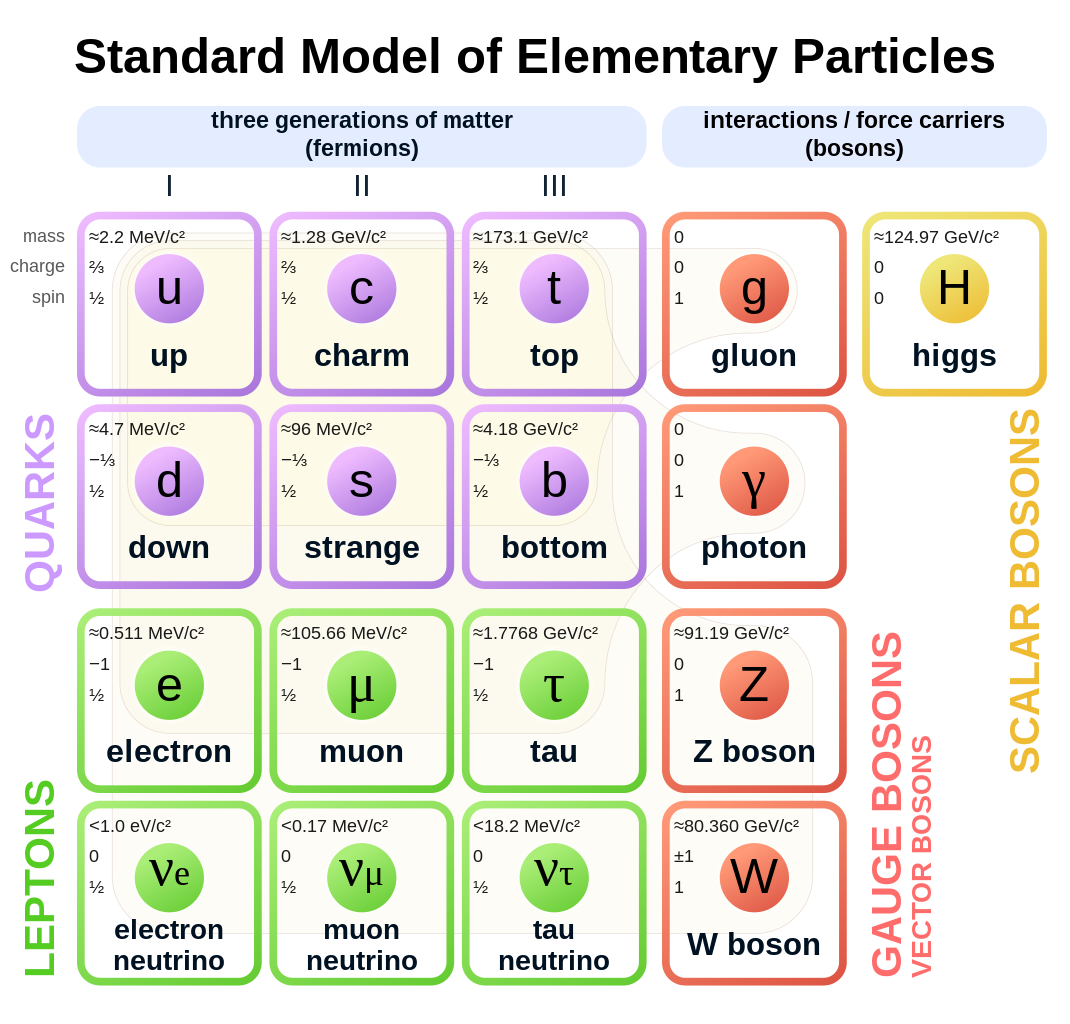
\includegraphics[width=0.5\linewidth]{plots/sm/Standard_Model_of_Elementary_Particles.svg.png}  \\
\caption[Elementary particles of the Standard Model]{Elementary particles of the Standard Model, including the most important quantum numbers.}
\label{fig:sm-particles}
\end{figure}

\subsection{Fermions}

According to the spin-statistics theorem, fermions respect the Pauli exclusion principle. Each fermion has a corresponding antiparticle. They can be classified further according to how they interact, or equivalently, by the charges they carry. There are six flavored quarks: up ($\PQu$), down ($\PQd$), charm ($\PQc$), strange ($\PQs$), top ($\PQt$), bottom ($\PQb$), and each has a corresponding antiparticle. They are divided into three generations, with each generation being heavier than the previous one. They are further grouped into up-type quarks ($\PQu$, $\PQc$, $\PQt$) and down-type quarks ($\PQd$, $\PQs$, $\PQb$). Quarks carry color charge, and hence interact via the strong interaction. The quarks are strongly bound to one another due to the phenomenon of color confinement. Therefore, they form color-neutral composite particles called hadrons, which can contain either a quark and an antiquark (mesons) or three quarks (baryons). Quarks also carry electric charge and weak isospin, allowing them to participate in electromagnetic and weak interactions.

In contrast to quarks, leptons do not carry a color charge and, therefore, do not participate in strong interactions. There are six flavored leptons: the electron (\Pe), the electron neutrino (\PGne), the muon (\PGm), the muon neutrino (\PGnGm), the tau (\PGt), and the tau neutrino (\PGnGt). Each lepton has a corresponding antiparticle. Leptons are also divided into three generations based on their masses. Since each member of a generation has a greater mass than the corresponding particle of any previous generation, the charged particles of the first generation do not decay. That's why all ordinary (baryonic) matter is made up of particles from the first generation.

The SM is a chiral theory, meaning that left-handed and right-handed fermions are treated differently. Under weak isospin $SU(2)$ transformations, the left-handed particles are weak-isospin doublets, whereas the right-handed particles are singlets. That means that all left-handed fermions have a weak isospin of $\pm 1/2$,  while the right-handed fermions have a weak isospin of 0. The charged left-handed leptons and the left-handed neutrinos of each generation are arranged as weak isospin doublets. The right-handed charged leptons are singlets. Right-handed neutrinos are not included in the original formulation of the SM. The weak hypercharge of the left-handed leptons is -1, while the right-handed leptons have a weak hypercharge of -2.

\subsection{Gauge bosons}

In the SM, gauge bosons are the force carriers that mediate the strong, weak, and electromagnetic fundamental interactions. The gauge bosons all have a spin of 1. Photons mediate the electromagnetic force between electrically charged particles. The photon is massless and is described well by the theory of quantum electrodynamics. The $\PWp$, $\PWm$, and $\PZz$ gauge bosons mediate the weak interactions, and are massive. The weak interactions involving the $\PWpm$ act only on left-handed particles and right-handed antiparticles. The electrically neutral $\PZz$ boson interacts with both left-handed particles and right-handed antiparticles. Since the $\PWpm$ bosons carry electric charges of $+1$ and $-1$, they also couple to the photon. The eight gluons mediate the strong interactions between color-charged particles (the quarks). Gluons are massless, and because they carry color charge themselves, they can interact with each other. The strong interaction is governed by the theory of Quantum Chromodynamics (QCD). The interactions of the SM are summarized in Figure~\ref{fig:sm-interactions}.

\begin{figure}[!htb]
\centering
\includegraphics[width=0.5\linewidth]{plots/sm/Standard_Model_–_All_Feynman_diagram_vertices.svg.png}  \\
\caption[Interactions of the Standard Model.]{Interactions of the Standard Model~\cite{Lindon:2746537}. Feynman diagrams in the SM are built from combinations of these vertices. $q$ is any quark, $g$ is a gluon, $X$ is any charged particle, $\gamma$ is a photon, $f$ is any fermion, $m$ is any particle with mass, $m_B$ is any boson with mass.}
\label{fig:sm-interactions}
\end{figure}

The combined symmetry group $SU(2)_L \times U(1)_Y$ gives rise to four gauge bosons. The symmetry group $U(1)_Y$ gives rise to $B$, and $SU(2)_L$ gives rise to $W^1$, $W^2$, and $W^3$. The physical bosons $\gamma$, $\PWp$, $\PWm$, and $\PZz$ are obtained by mixing these states due to the Higgs mechanism and are given by
\begin{equation}
\PWpm=\frac{1}{\sqrt(2)}\qty(W^1\mp i W^2)
\end{equation}
and
\begin{equation}
\mqty(\PGg \\ \PZ)=\mqty(\cos \theta_W & \sin \theta_W \\ -\sin \theta_W & \cos \theta_W)\cdot \mqty(B \\ W^3),
\end{equation}
where $\theta_W$ is the mixing angle, or Weinberg angle. The electric charge is determined by the weak isospin and
weak hypercharge by
\begin{equation}
Q=T_3+\frac{Y}{2}.
\end{equation}

Generally speaking, the weak interaction is responsible for processes such as radioactive decay. It has the ability to change flavors. In a neutron decay, for example, a down quark in the neutron emits a $\PWm$ boson, thereby changing into an up quark. The $\PWm$ boson then decays into an electron and an electron antineutrino. This process is not restricted to quarks within one generation. The probability of a transition from one flavour j quark to another flavour i quark is encoded in the Cabibbo–Kobayashi–Maskawa (CKM) matrix and is proportional to $\abs{V_{ij}}^2$. The three diagonal elements of the matrix are close to unity, which means decay processes within the same generation are favored, whereas the off-diagonal elements are small, especially for mixing with the third generation. The weak force also causes neutrino oscillations due to mismatch of quantum states of neutrinos when they propagate freely and when they take part in weak interactions. The Pontecorvo–Maki–Nakagawa–Sakata matrix (PMNS matrix) encodes the amplitude of the transitions between mass eigenstates and flavor eigenstates.

The strong interaction is referred to as Quantum Chromodynamics (QCD). QCD describes interactions between quarks mediated by gluons. It is a non-abelian gauge theory, with symmetry group $SU(3)$. The QCD analogue of electric charge is a property called color. Gluons are the force carriers of the theory, just as photons are for the electromagnetic force in quantum electrodynamics. The three kinds of charge in QCD are referred to as \emph{color charge}: red, green, blue, and their anticolors. The strong interaction is responsible for the nuclear force, which binds protons and neutrons in the nucleus. It also binds quarks together to form hadrons, including nucleons.

\subsection{Higgs Boson}

As mentioned in Section~\ref{spontaneous-symmetry-breaking}, the Higgs mechanism is responsible for the spontaneous symmetry breaking of the $SU(2)_L \times U(1)_Y$ gauge group, which generates mass for all the massive particles in the SM. The Higgs boson is a consequence of the Higgs field. The mass term arising from the Dirac Lagrangian (for any fermion $\psi$) is $-m\bar{\psi}\psi$, which is not invariant under the chiral electroweak symmetry. In addition, the W and Z bosons are massive, which is unlike what is predicted without symmetry breaking. To solve these problems, the Higgs mechanism is introduced. In the Standard Model, the Higgs field is a complex scalar field that forms an $SU(2)_L$ doublet:
\begin{equation}
\phi=\frac{1}{\sqrt{2}}\mqty(\phi^+ \\ \phi^0),
\end{equation}
where the superscripts + and 0 indicate the electric charge (Q) of the components. The weak hypercharge of both components is 1. The Higgs potential is symmetric with respect to the origin and has a non-trivial minimum. It is given by
\begin{equation}
V(\phi)=\mu^2\abs{\phi}^2+\lambda\abs{\phi}^4,
\end{equation}
where $\lambda>0,\mu^2<0$. In a unitarity gauge one can set $\phi^+=0$ and make $\phi^0$ real. Then $<\phi^0>=v$ is the non-vanishing vacuum expectation value of the Higgs field, which spontaneously breaks the symmetry of the electroweak model. It generates the Higgs boson $H$ with the mass
\begin{equation}
m_H=\sqrt{-2\mu^2}.
\end{equation}
The masses of the $\PW$ and $\PZ$ bosons are given by:
\begin{equation}
\begin{split}
m_\PW&=\frac{1}{2}gv \\
m_\PZ&=\frac{m_\PW}{\cos \theta_W}. \\
\end{split}
\end{equation}
Self-interaction terms of the Higgs boson are described by the coupling strength $\lambda$. The masses of the fermions are generated via the Yukawa couplings.

\subsection{Shortcomings of the Standard Model}

Although the SM is a very successful theory, it falls short of explaining all observations and open questions. It is, therefore, not regarded a \emph{theory of everything}, and it is agreed to be incomplete. Direct experimental evidence not explained in the SM include:
\begin{itemize}
\item \textbf{Gravity:} The SM does not account for gravity. That is perhaps one of the biggest challenges that physicists of our time face.
\item \textbf{Neutrino masses:} The phenomenon of neutrino oscillation suggest that the neutrinos have mass~\cite{Gonzalez_Garcia_2008}, in direct contradiction to the initial formulation of the SM which assumed that they have zero mass.
\item \textbf{Baryon asymmetry:} The SM does not explain the observed imbalance in baryonic matter and antibaryonic matter in the observable universe~\cite{Canetti_2012}. The CP violation accounted for in the SM is too small to explain why our universe is made mainly from matter and not almost equal amounts of matter and antimatter.
\item \textbf{Dark matter and dark energy:} The existence of dark matter is also not explained by the SM~\cite{Garrett_2011}. If it unclear yet if it is a particle, or a different kind of phenomenon, but if it is a particle, then the SM needs to be extended. The SM also does not account for the  universe's accelerating expansion as possibly described by dark energy.
\end{itemize}

In addition, the SM is seen by some to possess some conceptual deficiencies, such as:
\begin{itemize}
\item \textbf{Hierarchy problem:} The Higgs mechanism gives rise to the hierarchy problem if some new physics is present at high energy scales. If that is the case, severe fine tuning of the parameters is required between the bare mass of the Higgs boson, and the enormous loop corrections to the Higgs mass~\cite{Jegerlehner_2014}. A further discussion about this problem is given in Section~\ref{sec:naturalness}.
\item \textbf{Ad-hoc-ness:} The SM requires 26 numerical constants whose values are unrelated and arbitrary. It is also unclear why there are three generations of quark and leptons.
\item \textbf{Unification of forces:} the successful unification of the weak and electromagnetic forces suggest that a further unification with the strong force might be possible. This is referred to as a Grand-Unified-Theory (GUT) theory. In a GUT theory, the coupling strength of the interactions are expected to have the same magnitude at some high energy scale, which is not observed in the SM.
\end{itemize}

\clearpage
\section{Supersymmetry}

\glsreset{susy}\gls{susy} is a set of theories in which a symmetry that relates fermions and bosons is postulated~\cite{Peskin2019-bt,Garrett_2011,MARTIN_1998}. That is, a supersymmetry transformation turns a bosonic state into a fermionic state, and vice versa. The interest in \gls{susy} can be traced back to 1967, in which Coleman and Mandula proved a no-go theorem stating that spacetime and internal symmetries can only combine in a trivial way~\cite{PhysRev.159.1251}. This means that the charges associated with internal symmetries must always transform as Lorentz scalars. Also, there can be no change of the spin of particles. Fermions cannot change into bosons or vice versa. This was evaded in the 70s by different groups of physicists~\cite{GERVAIS1971632,HAAG1975257} with the discovery of \gls{susy}. It is done by loosening the restriction on the types of symmetries of a QFT, and in addition to Lie Algebras one can consider graded Lie Algebras whose operators anticommute. The first realistic supersymmetric version of the SM was proposed by Fayet and is known as the \gls{mssm}.

An operator $Q$ that generates transformations between bosonic and fermionic states must be an anti-commuting spinor, with
\begin{equation}
\begin{split}
Q\ket{\text{Boson}}=\ket{\text{Fermion}},\\
Q\ket{\text{Fermion}}=\ket{\text{Boson}}.
\end{split}
\end{equation}
Since $Q$ is a complex spinor, $Q^\dagger$ is also a symmetry generator. These operators carry spin angular momentum $1/2$, so that \gls{susy} is a spacetime symmetry. It has been demonstrated that the most general possibility of such operators is a collection of spin-$1/2$ operators with the anticommutation reations
\begin{equation}
\pb{Q^i_\alpha}{Q^{j\dagger}_\beta}=2\delta^{ij}\sigma^\mu_{\alpha\beta}P^\mu,
\end{equation}
with $i,j=1,\ldots,N$. All other anticommutation relations between the $Q$s and commutation relations between the $Q$s and $P$s vanish. In the following, the simplest case $N=1$ is considered. It is the simplest supersymmetric extension of the Poincaré algebra, or the Super-Poincaré algebra. The index $\alpha=1,2$ is the left-handed spinor components of the operator, and $P^\mu$ is the total energy-momentum. 

The single-particle states of a supersymmetric theory fall into irreducible representations of the supersymmetry algebra, called supermultiplets. Each supermultiplet contains both fermion and boson states, which are known as \emph{superpartners} of each other. The resulting commutation relation
\begin{equation}
\comm{Q}{P^2}=\comm{Q^{\dagger}_{\dot{\alpha}}}{P^2}=0
\end{equation}
implies that particles that are transformed into each other have the same eigenvalues of $P^2$, and therefore equal masses. The generators also commute with the generators of gauge transformations. That means that particles and their \emph{superpartners} must also share the same gauge charges.

Since we do not observe a bosonic superpartner to the electron, named \emph{selectron}, with the same mass as the electron, it is clear that supersymmetry must be a spontaneously broken symmetry. The specific mechanism of SUSY breaking is unknown, but usually, further terms that break SUSY explicitly are added by hand to the Lagrangian. However, since naturalness is often described as a motivation for introducing SUSY, it is required that the SUSY breaking terms still provide a solution to the hierarchy problem. This means that the effective Lagrangian contains only "soft" SUSY breaking, meaning that they violate SUSY but contain only mass terms and coupling parameters with a positive mass dimension.

\subsection{The Minimal Supersymmetric Standard Model}
\label{sec:MSSM}

The \glsreset{mssm}\gls{mssm} is an extension to the SM that realizes SUSY~\cite{MARTIN_1998}. It is minimal in regards to the number of new particle states and new interactions. In this extension, each of the known fundamental particles is in either a chiral or gauge supermultiplet, and must have a superpartner with spin differing by $1/2$ unit. The names for the spin-0 partners of the quarks and leptons are constructed by prepending an “s”, for scalar. They can therefore be called \emph{squarks} and \emph{sleptons}, or generally \emph{sfermions}. Their symbols normally contain a tilde ($\widetilde{\,\,\,}$). The MSSM contains two Higgs supermultiplets in order to prevent an electroweak gauge anomaly. The generic nomenclature for a spin-$1/2$ superpartner is to append “-ino” to the name of the SM particle, so the fermionic partners of the Higgs scalars are called \emph{higgsinos}. The vector bosons of the SM clearly reside in gauge supermultiplets. Their fermionic superpartners are generically referred to as \emph{gauginos}. The spin-$1/2$ superpartners of the electroweak gauge bosons are called \emph{winos} and \emph{binos}. Table~\ref{tab:chiral-supermultiplets} lists the chiral supermultiplets of the MSSM, while Table~\ref{tab:gauge-supermultiplets} lists the gauge supermultiplets of the MSSM.

\begin{table}[!htp]
	\centering
	\label{tab:chiral-supermultiplets}
		\caption{Chiral supermultiplets of the MSSM. The spin-0 fields are complex scalars, and the spin-$1/2$ fields are left-handed two-component Weyl fermions.
}
		%\vspace{1mm}
			\begin{tabular}{|l|c|c|c|}
\hline
Names                  & spin 0  & spin $1/2$ & $SU(3)_C,SU(2)_L,U(1)_Y$ \\ \hline\hline
\multirow{3}{*}{squarks, quarks} & $\qty(\widetilde{u}_L\,\widetilde{d}_L)$ & $\qty(u_L\,d_L)$ & $\qty(\mathbf{3},\mathbf{2},\frac{1}{6})$ \\  
                  & $\widetilde{u}^{*}_R$ & $u^{\dagger}_R$ & $\qty(\bar{\mathbf{3}},\mathbf{1},-\frac{2}{3})$ \\  
                  & $\widetilde{d}^{*}_R$ & $d^{\dagger}_R$  & $\qty(\bar{\mathbf{3}},\mathbf{1},\frac{1}{3})$ \\ \hline
\multirow{2}{*}{sleptons, leptons} & $\qty(\widetilde{\nu}\,\widetilde{e}_L)$ & $\qty(\nu\,e_L)$ & $\qty(\mathbf{1},\mathbf{2},-\frac{1}{2})$  \\ 
                  & $\widetilde{e}^{*}_R$ & $e^{\dagger}_R$ & $\qty(\mathbf{1},\mathbf{1},1)$ \\ \hline
\multirow{2}{*}{Higgs, higginos} & $\qty(H^{+}_u\,H^{0}_u)$ & $\qty(\widetilde{H}^{+}_u\,\widetilde{H}^{0}_u)$ & $\qty(\mathbf{1},\mathbf{2},+\frac{1}{2})$ \\ 
                  & $\qty(H^{0}_d\,H^{-}_d)$ & $\qty(\widetilde{H}^{0}_d\,\widetilde{H}^{-}_d)$ & $\qty(\mathbf{1},\mathbf{2},-\frac{1}{2})$ \\ \hline
\end{tabular}
\end{table}

\begin{table}[!htp]
	\centering
	\label{tab:gauge-supermultiplets}
		\caption{Gauge supermultiplets of the MSSM.
}
		%\vspace{1mm}
			\begin{tabular}{|l|c|c|c|}
\hline
Names                  & spin $1/2$  & spin 1 & $SU(3)_C,SU(2)_L,U(1)_Y$ \\ \hline \hline 
gluino, gluon & $\PSg$ & $\Pg$ & $\qty(\mathbf{8},\mathbf{1},0)$ \\  
                   \hline
winos, $\PW$ bosons & $\PSWpm\,\PSW^0$ & $\PWpm\,\PW^0$ & $\qty(\mathbf{1},\mathbf{3},0)$  \\  \hline
bino, $B$ boson & $\widetilde{B}^0$ & $B^0$ & $\qty(\mathbf{1},\mathbf{1},0)$ \\ 
                   \hline
\end{tabular}
\end{table}

The superpartners listed in Tables~\ref{tab:chiral-supermultiplets} and~\ref{tab:gauge-supermultiplets} are not necessarily the mass eigenstates of the theory. Electroweak symmetry breaking and SUSY breaking can cause mixing between the electroweak gauginos and the higgsinos, and within the various sets of squarks and sleptons and Higgs scalars that have the same electric charge. The gluino cannot mix since it is a color octet fermion and therefore does not have the appropriate quantum numbers to mix with any other particle. The neutral higgsinos, $\widetilde{H}^{0}_u$ and $\widetilde{H}^{0}_d$, and the neutral gauginos, $\widetilde{B}^0$ and $\PSW^0$, mix into four mass eigenstates called \emph{neutralinos}. The charged higgsinos, $\widetilde{H}^{+}_u$ and $\widetilde{H}^{-}_d$, and winos, $\widetilde{W}^+$ and $\widetilde{W}^-$, mix to form two mass eigenstates with charge $\pm 1$ called \emph{charginos}. The neutralinos are labeled $\PSGczDo,\PSGczDt,\PSGczDT,\PSGczDf$ in increasing order of mass, and the charginos are labeled $\PSGcpmDo,\PSGcpmDt$, also in increasing order of mass. In the gauge-eigenstate basis $\qty(\widetilde{B},\PSW^0,\widetilde{H}^{0}_d,\widetilde{H}^{0}_u)$, the neutralino mass matrix is given by:
\begin{equation}
M_N=\mqty(M_1 & 0 & -c_\beta s_W m_Z & s_\beta s_W m_Z\\
0 & M_2 &  c_\beta c_W m_Z & -s_\beta c_W m_Z \\
-c_\beta s_W m_Z & c_\beta c_W m_Z & 0 & -\mu\\
s_\beta s_W m_Z & -s_\beta c_W m_Z & -\mu & 0),
\end{equation}
where masses $M_1$ and $M_2$ are the $U(1)$ and $SU(2)$ gaugino masses, $\mu$ is the higgsino mass parameter, and $\tan \beta=v_u/v_d$ is the ratio of the vacuum
expectation values of the two neutral Higgs fields which break the electroweak symmetry. Here, $s_\beta=\sin\beta$, $c_\beta=\cos\beta$ and $s_W,c_W$ are the sine and cosine of the electroweak mixing
angle $\theta_W$. The mixing of the charged gauginos and charged higgsinos is given by the matrix:
\begin{equation}
M_C=\mqty(M_2 & \frac{1}{\sqrt{2}}gv_u\\
\frac{1}{\sqrt{2}}gv_d & \mu),
\end{equation}
where $g$ is the $SU(2)$ gauge coupling.

A neutralino state can approximate a particular gaugino or higgsino state. If $\abs{M_1}$ and $\abs{M_2}$ are small compared to $m_Z$ and $\abs{\mu}$, then $\PSGczDo$ would be nearly a pure photino. If $\abs{M_1}$ and $m_Z$ are small compared to $\abs{M_2}$ and $\abs{\mu}$, then $\PSGczDo$ would be nearly a pure bino. If $\abs{M_2}$ and $m_Z$ are small compared to $\abs{M_1}$ and $\abs{\mu}$ then the lightest chargino pair and neutralino would constitute a triplet of roughly
mass-degenerate pure winos. Finally, if $\abs{\mu}$ and $m_Z$ are small compared to $\abs{M_1}$ and $\abs{M_2}$, then the lightest chargino pair and neutralino would be nearly pure higgsino states. These cases lead to strikingly different phenomenology.

For reasons such as proton stability, suppression of neutrino masses, and the accidental globel $B-L$ symmetry of the SM that is not automatically conserved in a generic supersymmetric extension of the SM, an addition symmetry called R-parity is added to the MSSM. It is defined as
\begin{equation}
R=\qty(-1)^{3(B-L)+2S},
\end{equation}
where B is baryon number, L is lepton number, and S is the spin. This implies that all the particles of the SM have even R-parity, whereas their corresponding superpartners have odd R-parity. Moreover,
R-parity invariance also implies that the lightest supersymmetric particle (LSP) is absolutely stable. Usually, the lightest neutralino is assumed to be the LSP, and it makes an attractive candidate for dark matter. It is often called a \gls{wimp}.

There are three principal motivations for the MSSM. We have encountered the first one, and that is that the LSP is a good dark matter candidate~\cite{Garrett_2011}. The second motivation is that if the superpartners are near the TeV scale, then measured gauge couplings of the three gauge groups unify at high energies~\cite{PhysRevD.24.1681}. The third motivation for the MSSM, and also why it was originally proposed, is that it could solve the hierarchy problem~\cite{DIMOPOULOS1981150}. This problem is described further in Section~\ref{sec:naturalness}.

Since the MSSM has more than 100 parameters in addition to the SM, it makes phenomenological analysis quite impractical. Therefore, reasonable constraints can be imposed on the MSSM in order to reduce the number of free parameters. Such a selection of assumptions is done in a submodel of the MSSM called the phenomenological MSSM (pMSSM)~\cite{djouadi1999minimal,Berger_2009}. The following assumptions define the pMSSM:
\begin{itemize}
\item no new source of CP-violation;
\item no flavour changing neutral currents;
\item first and second generation universality.
\end{itemize}
These assumption reduce the number of SUSY parameters to 19.


\subsection{Naturalness}
\label{sec:naturalness}

One of the motivations for SUSY, and for the MSSM in particular, is that it is able to solve the hierarchy problem of the Higgs boson's mass. This problem is closely related to fine-tuning and naturalness. The physical principle of \emph{naturalness} was articulated by ’t Hooft and states that a small parameter is natural only when a symmetry is gained as it is set to zero~\cite{tHooft:1980xss,Seiberg_1993}. That means that in QFT, if a bare parameter is unnaturally set to zero, radiative corrections lead to a renormalized non-zero value. If a small renormalized value is desired without a symmetry, the bare value has to be fine-tuned.

Mathematically speaking, the problem is related to quantum corrections that the mass of the Higgs boson (squared) receives from the virtual effects of every particle that couples, directly or indirectly, to the Higgs field. For a Dirac fermion $f$ that couples to the Higgs field via a term in the Lagrangian $-\lambda_f H \bar{f}f$, the mass squared of the Higgs boson receives a correction of
\begin{equation}
\Delta m^2_H = -\frac{\abs{\lambda_f}^2}{8\pi^2}\Lambda^2_{\mathrm{UV}}+\ldots,
\end{equation} 
where $\lambda_f$ is the Yukawa coupling and $\Lambda^2_{\mathrm{UV}}$ is an ultraviolet momentum cutoff used to regulate the loop integral. Each of the leptons and quarks of the SM contributes such a correction, with the top quark being the largest contribution with $\lambda_f\approx 0.94$~\cite{MARTIN_1998}. If the cutoff is of the order of $M_P$, then the quantum correction is 30 orders of magnitude larger than the required value $m^2_H\approx-\qty(92.9\GeV)^2$ without radiative corrections. This, for some physicists, makes it difficult to understand why $m^2_H$ is so small. In other words, it seems unlikely that such large contributions will add up to a small number, and it is an example of fine-tuning.

If SUSY is present, these large contributions can be avoided by cancellations between fermionic loops and loops from complex scalar particles. For a scalar particle $S$ with mass $m_S$ and a Lagrangian term $-\Lambda_S\abs{H}^2\abs{S}^2$, the correction is given by
\begin{equation}
\Delta m^2_H = \frac{\lambda_S}{16\pi^2}\left[\Lambda^2_{\mathrm{UV}} -2m_S^2\ln(\Lambda_{\mathrm{UV}}/m_S) \ldots\right].
\end{equation}
Since in the MSSM, each of the quarks and leptons of the SM is accompanied by two complex scalars with $\lambda_S=\abs{\lambda_f}^2$, the $\Lambda^2_{\mathrm{UV}}$ contributions neatly cancel. While this cancellation is true for unbroken SUSY, broken SUSY scenarios will require some amount of fine-tuning. The amount of fine-tuning in the MSSM can be quantified~\cite{Feng_2013,PhysRevD.58.096004}. If one requires a reasonable amount of fine-tuning, that puts constraints on the phenomenology of the MSSM. A 10\% level of fine-tuning will require the existence of one pair of charginos and two neutralinos with a maximum mass of $200-300\GeV$~\cite{natural-SUSY,BARBIERI198863,Antusch_2013,Papucci_2012}. In particular, natural SUSY scenarios correspond to a higgsino parameter space of $\abs{\mu}\lesssim 150-200\GeV$~\cite{Baer_2012}.
